\section{Experimentos y resultados}
\label{sec:experimentos}

Los experimentos usan el silver standard de 43 preguntas; E12 usa la versi\'on ampliada con 17 documentos adicionales y cada tabla lo indica. La configuraci\'on se eligi\'o con el silver completo, as\'i que los resultados son exploratorios. Cada subsecci\'on reporta el montaje en una frase, la tabla y la decisi\'on; el detalle del montaje est\'a en la Secci\'on~\ref{sec:metodo}.

\subsection{Arco experimental}

Los experimentos no forman una rejilla: siguen un arco de seis estaciones, y cada una se abre con la pregunta que deja la anterior.

\begin{itemize}
\item \textbf{L\'inea base sobre el piloto.} Limpieza, segmentaci\'on y n\'umero de fragmentos con e5-base y 1.932 documentos (Subsecciones \emph{Limpieza} a \emph{Segmentaci\'on y tama\~no del contexto}). El piloto deja un techo alto, Recall@10 de 0,947, y decisiones tomadas por coste y consistencia, no por significancia estad\'istica.
\item \textbf{Modelos peque\~nos e H1.} E4 compara cuatro generadores de 1B a 3B con la misma evidencia recuperada (Subsecci\'on \emph{Modelos generativos}). H1 se refuta: el tama\~no no ordena la calidad; gemma2:2b gana en correcci\'on y citas y llama3.2:1b se abstiene en el 73,7\,\% de las preguntas respondibles.
\item \textbf{Crisis de escala.} E6 repite el pipeline sobre el corpus completo, 161.868 documentos (Subsecci\'on \emph{Codificadores y escala}). Recall@10 cae de 0,947 a 0,684 y nDCG de 0,909 a 0,594 sin que la latencia cambie; la ca\'ida reorganiza el resto del trabajo.
\item \textbf{Rescate h\'ibrido.} BM25, bge-m3, \texttt{ef}=800, la uni\'on densa y dispersa y el reordenador recuperan parte de la p\'erdida (Subsecciones \emph{Codificadores y escala} y \emph{Reordenamiento}). La fusi\'on RRF se rechaza con el silver ampliado y la uni\'on reordenada se adopta para el despliegue.
\item \textbf{Ablaciones negativas.} Las fases 6 y 7 y la inyecci\'on de instrucciones prueban mejoras que no superan la referencia (Subsecciones \emph{Inyecci\'on de instrucciones} y \emph{Prompts y mejoras rechazadas}). Se reportan para acotar el espacio, no para justificar la configuraci\'on.
\item \textbf{Arquitectura ganadora y reservado.} La instancia final se eval\'ua con la compuerta de dominio, RAGAS y el conjunto reservado de 20 preguntas directas y 5 negativas (Subsecciones \emph{Compuerta de dominio} a \emph{Conjunto reservado}). Es la evaluaci\'on de cierre y se reporta tal como sale, incluidas las cifras que empeoran la l\'inea base.
\end{itemize}

El orden importa: las estaciones iniciales se deciden con el silver exploratorio y el conjunto reservado se usa al final para comparar la configuraci\'on desplegada; las cifras de una estaci\'on no se trasladan a otra. Cada subsecci\'on indica con qu\'e conjunto se midi\'o.

\subsection{Limpieza}

Se construyeron cuatro \'indices sobre el piloto con 30 preguntas, e5-base, $k=10$ y tres repeticiones. La Tabla~\ref{tab:limpieza} muestra el resultado. Ninguna comparaci\'on pareada contra V0 excluye cero tras la correcci\'on de Bonferroni sobre 21 pruebas. V2 toca el l\'imite inferior en cuatro m\'etricas, compatible con una mejora peque\~na o con ausencia de efecto. Se adopta V2 por tres razones no estad\'isticas: la consistencia de la estimaci\'on en todas las m\'etricas, el coste nulo en consulta y la eliminaci\'on de 68 p\'aginas de error que de otro modo entrar\'ian al \'indice.

\begin{table}[t]
\centering
\footnotesize
\caption{Limpieza sobre el piloto (30 preguntas, e5-base, $k=10$).}
\label{tab:limpieza}
\setlength{\tabcolsep}{4pt}
\begin{tabular}{lrrrrr}
\toprule
Variante & P@1 & Hit@5 & Recall@10 & MRR & nDCG \\
\midrule
V0 crudo & 0,733 & 0,833 & 0,833 & 0,775 & 0,790 \\
V1 sin p\'aginas de error & 0,767 & 0,833 & 0,833 & 0,800 & 0,809 \\
V2 normalizaci\'on & \textbf{0,833} & \textbf{0,900} & \textbf{0,900} & \textbf{0,867} & \textbf{0,875} \\
V3 V2 + dedup & 0,800 & 0,867 & 0,867 & 0,833 & 0,842 \\
\bottomrule
\end{tabular}
\end{table}

\begin{figure}[t]
\centering
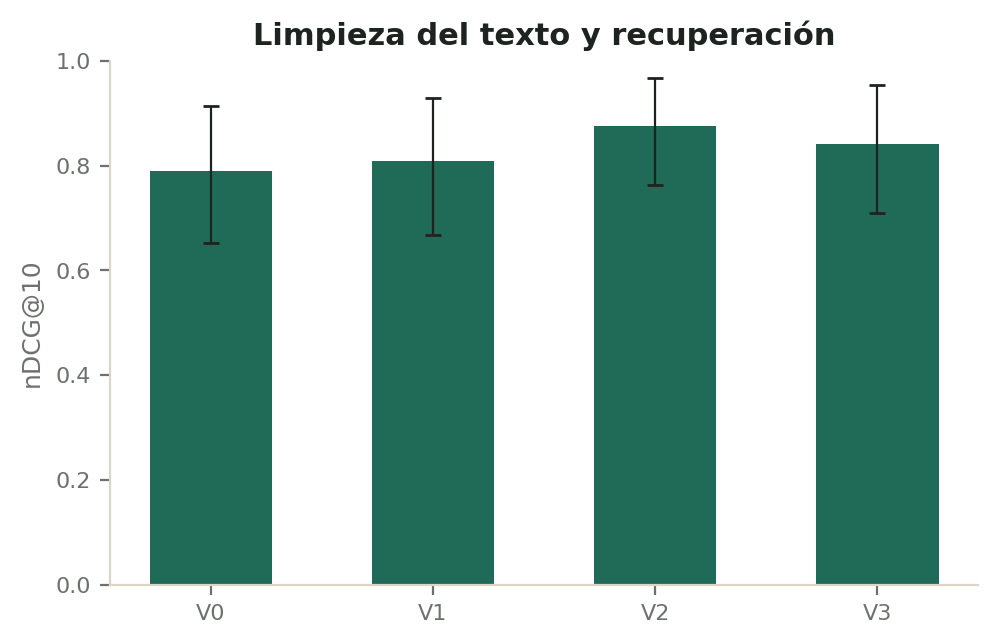
\includegraphics[width=\columnwidth]{limpieza_comparacion.png}
\caption{Comparaci\'on de variantes de limpieza sobre el piloto.}
\label{fig:limpieza}
\end{figure}


\subsection{Segmentaci\'on y tama\~no del contexto}

E1 compar\'o chunking fijo de 1000 caracteres con 150 de solape contra segmentaci\'on por oraciones de 384 caracteres. La Tabla~\ref{tab:e1} muestra estimaciones puntuales favorables al fijo en todas las m\'etricas de calidad, pero ning\'un intervalo pareado excluye cero: nDCG $-0,071$ (IC $[-0,221;\,0,025]$), recall $-0,067$ (IC $[-0,233;\,0,000]$) y P@1 $-0,067$ (IC $[-0,233;\,0,114]$) para oraciones menos fijo. La \'unica diferencia concluyente es la latencia: el fijo es 3,65 ms m\'as r\'apido (IC $[2,25;\,4,97]$). Se mantiene el fijo por la direcci\'on consistente y el coste, no por una mejora de calidad demostrada.

\begin{table}[t]
\centering
\footnotesize
\caption{E1: chunking fijo contra oraciones (30 preguntas).}
\label{tab:e1}
\begin{tabular}{lrrrrr}
\toprule
Variante & P@1 & Hit@5 & Recall@10 & nDCG & p50 \\
\midrule
Fijo 1000/150 & \textbf{0,833} & \textbf{0,900} & \textbf{0,900} & \textbf{0,875} & \textbf{38,5 ms} \\
Oraciones 384/1 & 0,767 & 0,833 & 0,833 & 0,804 & 42,1 ms \\
\bottomrule
\end{tabular}
\end{table}

\begin{figure}[t]
\centering
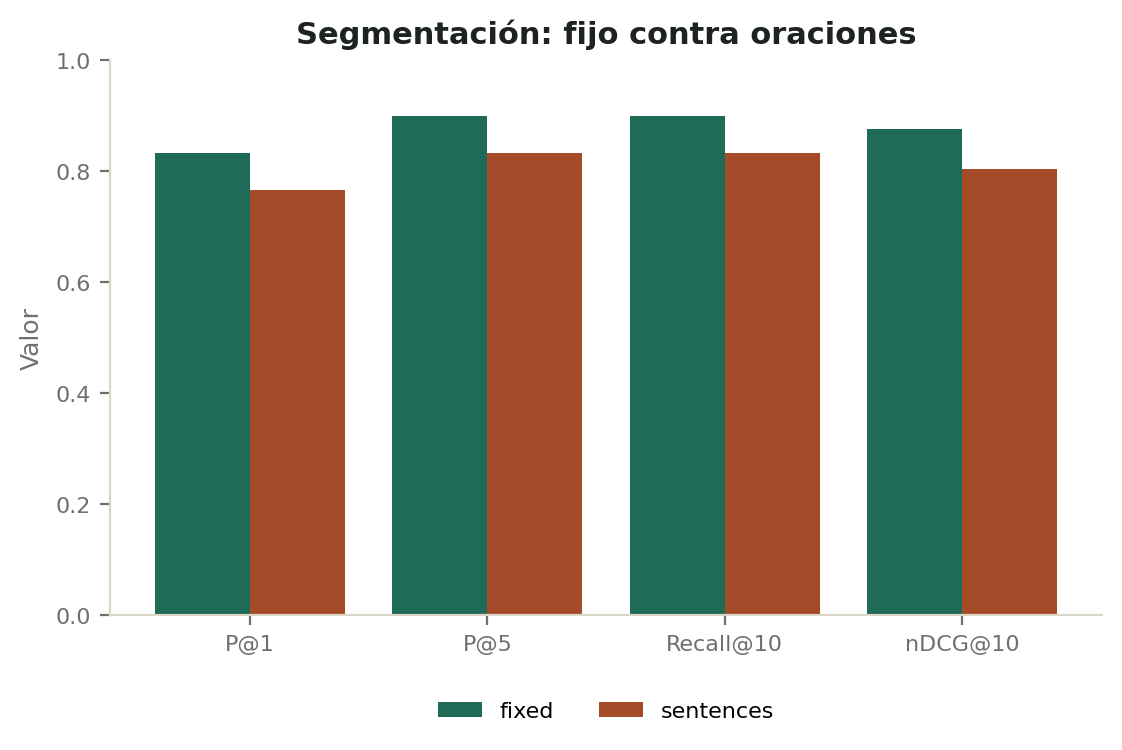
\includegraphics[width=\columnwidth]{e1_chunking.png}
\caption{Segmentaci\'on: fijo contra oraciones.}
\label{fig:e1}
\end{figure}


E2 ablacion\'o el n\'umero de fragmentos. Con el silver del piloto, el documento relevante est\'a siempre en el top-3, as\'i que $k=3$, 5 y 10 devuelven las mismas m\'etricas de calidad. La \'unica diferencia significativa es la latencia: $k=3$ tarda 1,64 ms menos que $k=10$ y $k=5$ tarda 0,94 ms menos. Se fija $k=5$ como margen para preguntas comparativas que no est\'an en el conjunto, sabiendo que el coste es m\'as contexto en generaci\'on, no m\'as latencia de recuperaci\'on.

\begin{figure}[t]
\centering
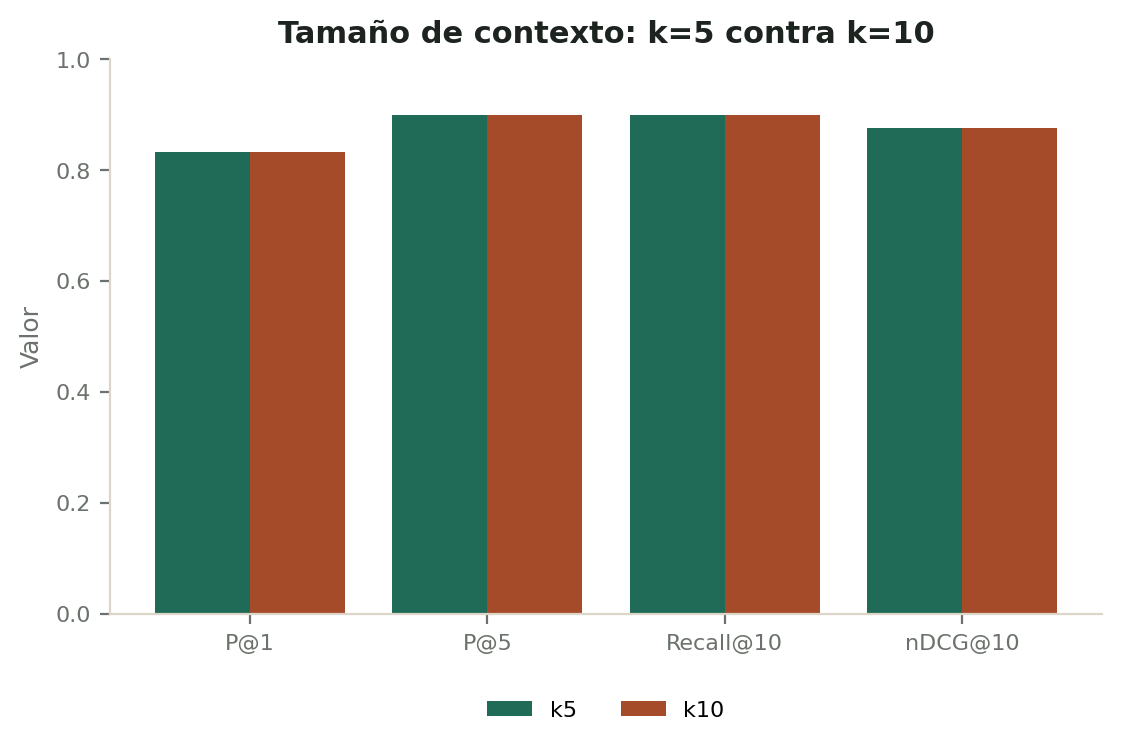
\includegraphics[width=\columnwidth]{e2_k5_vs_k10.png}
\caption{Tama\~no del contexto: $k=5$ contra $k=10$.}
\label{fig:e2}
\end{figure}


\begin{figure}[t]
\centering
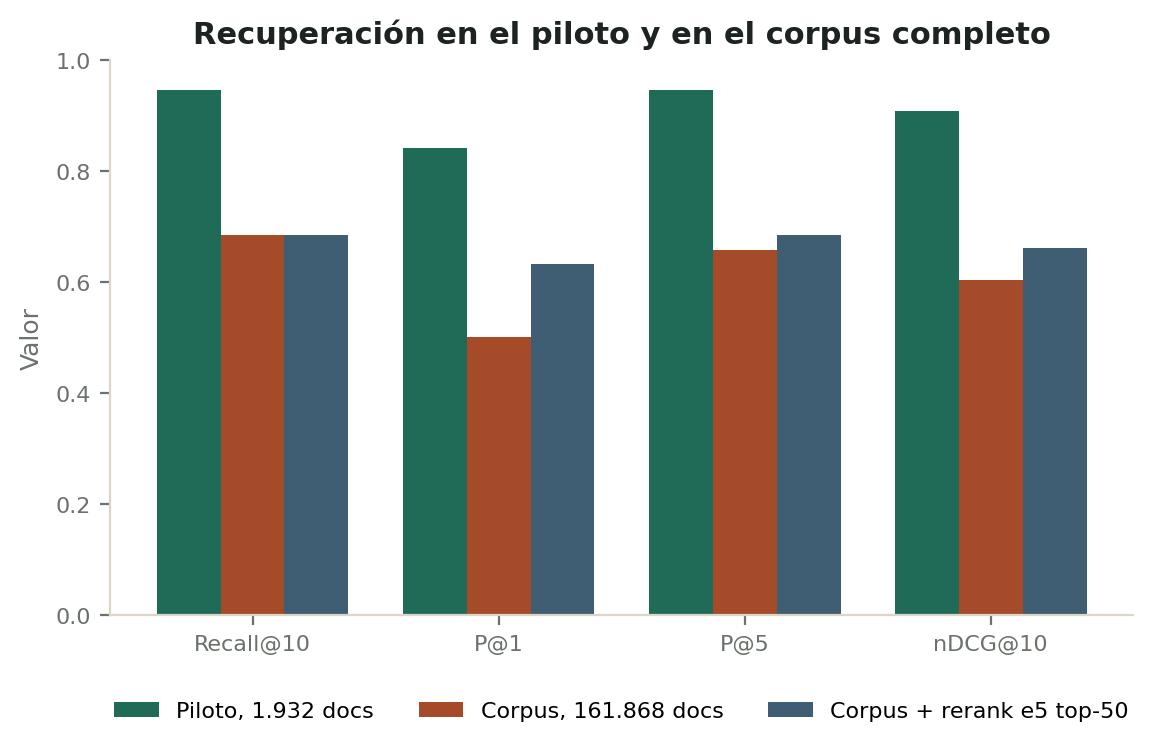
\includegraphics[width=\columnwidth]{escala_e6_e7.png}
\caption{Recuperaci\'on con e5-base sobre el silver de 38 preguntas respondibles: piloto (1.932 documentos), corpus completo (161.868 documentos) y corpus con reranker sobre el top-50. El piloto y el corpus usan \'indices separados.}
\label{fig:escala}
\end{figure}

\subsection{Codificadores y escala}

E3 compar\'o e5-base con qwen3-embedding:8b sobre el piloto, con 18 preguntas de desarrollo. qwen3 recupera mejor: Recall@10 perfecto y 6,4 puntos m\'as de nDCG. El problema es el coste. e5-base index\'o el corpus completo en 2 h 41 min medidos en la RX 9070 XT. qwen3-embedding:8b no se index\'o entero: las 23 horas son una extrapolaci\'on desde el rendimiento por lote, no un tiempo medido. Se adopta e5-base para la ingesta y qwen3 queda como comparaci\'on documentada.

E6 midi\'o el mismo pipeline sobre el corpus completo. La Figura~\ref{fig:escala} muestra la ca\'ida. La ca\'ida es el hallazgo m\'as importante del trabajo: con el mismo codificador y los mismos par\'ametros de \'indice en colecciones separadas, y las mismas 38 preguntas, Recall@10 pasa de 0,947 a 0,684 y nDCG de 0,909 a 0,594 al crecer de 1.932 a 161.868 documentos. La latencia no explica la ca\'ida (40 ms contra 42 ms). El experimento observa la ca\'ida al aumentar la escala; no separa competencia entre fragmentos, truncamiento del texto ni segmentaci\'on.

\begin{table}[t]
\centering
\footnotesize
\caption{E6: piloto contra corpus completo con e5-base (38 preguntas).}
\label{tab:e6}
\begin{tabular}{lrrrrr}
\toprule
Corpus & Recall@10 & P@1 & Hit@5 & nDCG & Span \\
\midrule
Piloto (1.932 docs) & \textbf{0,947} & \textbf{0,842} & \textbf{0,947} & \textbf{0,909} & \textbf{0,895} \\
Completo (161.868) & 0,684 & 0,474 & 0,658 & 0,594 & 0,658 \\
\bottomrule
\end{tabular}
\end{table}

E8 y E10 buscaron un recuperador mejor. BM25 sparse sube el recall a 0,763 y es ocho veces m\'as r\'apido, pero su techo de cobertura es bajo. bge-m3 llega a 0,842 de Recall@10 y 0,708 de nDCG, y recupera el ingl\'es de 0,111 a 0,667. La Tabla~\ref{tab:codificadores} resume.

\begin{table}[t]
\centering
\footnotesize
\caption{E10: recuperadores sobre el corpus completo (38 preguntas).}
\label{tab:codificadores}
\begin{tabular}{lrrrrr}
\toprule
M\'etodo & Recall@10 & P@1 & Hit@5 & nDCG & p50 \\
\midrule
Denso e5 & 0,684 & 0,500 & 0,658 & 0,604 & 48 ms \\
BM25 sparse & 0,763 & \textbf{0,684} & 0,737 & \textbf{0,727} & \textbf{7 ms} \\
bge-m3 & \textbf{0,842} & 0,553 & \textbf{0,816} & 0,708 & 56 ms \\
\bottomrule
\end{tabular}
\end{table}

E11 ajust\'o \texttt{ef} y prob\'o la fusi\'on con BM25. \texttt{ef}=800 sube el recall 2,6 puntos y el nDCG 1,3 con 6 ms m\'as. La fusi\'on 0,5/0,5 empata en recall y sube nDCG 6,9, P@1 13,2 y cobertura de span 5,3. Con el silver de un solo relevante la fusi\'on parec\'ia ganar. E12 repiti\'o la comparaci\'on con el silver ampliado: el denso recupera m\'as documentos nuevos (Recall@10 0,921 contra 0,890 y nDCG 0,827 contra 0,804). E12 se queda con la base densa, \texttt{ef}=800, sin fusi\'on; la ruta desplegada despu\'es es la uni\'on h\'ibrida, elegida sobre el conjunto de desarrollo.

\subsection{Solr como backend de recuperaci\'on}

Solr 9 se despleg\'o como un servicio m\'as del stack de Swarm, con imagen, puerto, CPU y memoria parametrizados. El \'indice replica los 618.286 fragmentos con un esquema de 13 campos y b\'usqueda \texttt{edismax} sobre \texttt{text} y \texttt{title}$^2$. La Tabla~\ref{tab:solr} compara el mismo silver de 38 preguntas. Solr con BM25 iguala el recall y el Hit@5 del BM25 de Milvus, pero pierde P@1 y nDCG. Con bge-m3, Solr alcanza 0,605 de recall, por debajo del denso de Milvus (0,842); la diferencia es consistente con el \'indice HNSW por defecto de Solr, que no se ajust\'o, y no con el embedding, que es el mismo. El backend es sustituible, pero el denso de Milvus sigue siendo la mejor opci\'on para la recuperaci\'on inicial; una comparaci\'on justa de Solr denso exige ajustar \texttt{hnswBeamWidth} y reconstruir el \'indice. El servicio se levanta con \texttt{scripts/deploy\_solr.sh} y la API de la demo corre en el puerto 8011 con \texttt{RETRIEVER=solr}.

\begin{table}[t]
\centering
\footnotesize
\setlength{\tabcolsep}{3pt}
\caption{Solr contra los recuperadores de Milvus sobre las 38 preguntas respondibles.}
\label{tab:solr}
\begin{tabular}{lrrrrr}
\toprule
Recuperador & Recall@10 & P@1 & Hit@5 & nDCG & p50 \\
\midrule
Solr BM25 & 0,763 & 0,526 & 0,737 & 0,652 & 37 ms \\
Solr bge-m3 & 0,605 & 0,395 & 0,579 & 0,510 & 109 ms \\
Milvus BM25 & 0,763 & \textbf{0,684} & 0,737 & \textbf{0,727} & \textbf{7 ms} \\
Milvus bge-m3 & \textbf{0,842} & 0,553 & \textbf{0,816} & 0,708 & 56 ms \\
\bottomrule
\end{tabular}
\end{table}

\subsection{Reordenamiento}

E7 midi\'o el cross-encoder sobre el top-50 con e5 en el corpus completo: P@1 sube de 0,474 a 0,632 y nDCG de 0,594 a 0,661, pero el Recall@10 se queda en 0,684; Hit@5 sube de 0,658 a 0,684 y la cobertura de span de 0,632 a 0,658. El coste es de 3,1 s por consulta. La mejora de orden no compensa el coste si se reordena tanto.

El denso a $k=10$ recupera 0,912 de recall y 0,818 de nDCG. Con bge-m3 se prob\'o reordenar 5 y 20 candidatos. La Tabla~\ref{tab:rerank} muestra que el top-20 baja el recall a 0,864 y el Hit@5 a 0,921, mientras que el top-5 mantiene 0,895 de recall y 0,947 de Hit@5, y sube el nDCG a 0,865 y el P@1 a 0,868 con 1,30 s. La tabla mide el reordenador en CPU; en la configuraci\'on final corre en GPU, con 0,68 s para 50 pares. La configuraci\'on final no reordena el top-5 denso: reordena la uni\'on con BM25 y recorta a 10.

\begin{table}[t]
\centering
\footnotesize
\caption{Reordenamiento con bge-m3 (38 preguntas).}
\label{tab:rerank}
\begin{tabular}{lrrrrr}
\toprule
Configuraci\'on & Recall & nDCG & P@1 & Hit@5 & p50 \\
\midrule
Denso top-5 & 0,895 & 0,809 & 0,737 & 0,947 & 0,10 s \\
Rerank top-5 & 0,895 & \textbf{0,865} & \textbf{0,868} & \textbf{0,947} & 1,30 s \\
Rerank top-20 & 0,864 & 0,853 & \textbf{0,868} & 0,921 & 5,46 s \\
\bottomrule
\end{tabular}
\end{table}


\subsection{Modelos generativos}

E4 compar\'o cuatro modelos con la misma evidencia: 19 preguntas respondibles y 5 sin respuesta, tres repeticiones, anotaci\'on humana ciega de la primera repetici\'on. La anotaci\'on cubre 18 de las 19 respondibles. La Tabla~\ref{tab:e4} muestra las medias de los dos anotadores en escala de 0 a 3. gemma2:2b gana en correcci\'on, citas y abstenci\'on. La fidelidad no se usa para el veredicto porque su acuerdo es $\kappa=0,12$. qwen2.5:1.5b es el m\'as r\'apido pero no cita en el 89,5\,\% de los casos. llama3.2:3b cita la mitad de las veces. llama3.2:1b se abstiene en el 73,7\,\% de las preguntas respondibles y no se recomienda.

\begin{table}[t]
\centering
\footnotesize
\caption{E4: anotaci\'on humana (0 a 3) y conducta autom\'atica.}
\label{tab:e4}
\begin{tabular}{lrrrr}
\toprule
Modelo & Correcci\'on & Citas & Abstenci\'on & Sin citas \\
\midrule
gemma2:2b & \textbf{2,81} & \textbf{2,67} & \textbf{2,89} & \textbf{0,0\,\%} \\
qwen2.5:1.5b & 2,31 & 0,00 & 2,81 & 89,5\,\% \\
llama3.2:3b & 2,22 & 0,86 & 2,69 & 56,1\,\% \\
llama3.2:1b & 0,42 & 0,28 & 1,61 & 15,8\,\% \\
\bottomrule
\end{tabular}
\end{table}

La hip\'otesis H1, que esperaba que llama3.2:3b superara a los dem\'as en correcci\'on y citas, se refuta. La evidencia recuperada es la misma entre modelos; lo que cambia es el generador. La comparaci\'on fij\'o la familia de modelos peque\~nos. El generador final es gemma4:e4b, que no estaba en E4: se adopt\'o despu\'es por contexto largo y MTP, no por ganar una comparaci\'on directa, y se valid\'o en la corrida final.

Se prob\'o un generador local de 27B (\texttt{qwen3.8:docs-32k-q3\_k\_s}, Q3) con el mismo pipeline y el mismo prompt. En test obtiene 0,917 de exactitud, 0,489 de cobertura, 0,657 de correcci\'on RAGAS y 10,3 s de mediana, frente a 0,917, 0,522, 0,652 y 1,2 s del 4B. El modelo grande no mejora de forma apreciable las m\'etricas y multiplica la latencia por ocho; el 4B se queda como generador desplegado.

\subsection{Inyecci\'on de instrucciones}

E5 insert\'o instrucciones expl\'icitas en cinco documentos sint\'eticos por modelo. Es una prueba exploratoria: no cubre el generador final ni demuestra robustez general. Dos de los tres modelos las ignoraron. gemma2:2b obedeci\'o una de cinco y a\~nadi\'o la palabra pedida a una respuesta por lo dem\'as correcta. La regla de dise\~no que sale de aqu\'i es que el prompt debe delimitar la evidencia y ordenar expl\'icitamente ignorar instrucciones internas, y esa orden debe repetirse despu\'es del bloque de contexto.

\begin{table}[t]
\centering
\footnotesize
\caption{E5: instrucciones inyectadas en el texto recuperado.}
\label{tab:e5}
\begin{tabular}{lrrr}
\toprule
Modelo & Obedeci\'o & Respondi\'o el hecho & Se abstuvo \\
\midrule
gemma2:2b & 1/5 & 4/5 & 0/5 \\
llama3.2:3b & 0/5 & 5/5 & 0/5 \\
qwen2.5:1.5b & 0/5 & 5/5 & 0/5 \\
\bottomrule
\end{tabular}
\end{table}


\subsection{Prompts y mejoras rechazadas}

La fase 6 prob\'o cuatro mejoras sobre la configuraci\'on de referencia y la fase 7 prob\'o diversidad. La referencia de estas fases era el top-5 denso con reranker; la uni\'on con BM25 se adopt\'o despu\'es, en el conjunto reservado. Ninguna de las variantes de las fases 6 y 7 supera a esa referencia. La Tabla~\ref{tab:fases} resume. El filtro por score pierde recall; reordenar el top-20 pierde Hit@5 y multiplica la latencia; la expansi\'on de consulta baja el recall y el nDCG; el prompt v4 no mejora la cobertura de tokens; y MMR baja el recall 8 puntos. El prompt v4 entreg\'o 37 de 38 y 25 de 37 de cobertura de tokens, sin mejora. Todas se rechazan y la configuraci\'on se mantiene.

\begin{table*}[t]
\centering
\footnotesize
\caption{Fases 6 y 7: variantes probadas sobre 38 preguntas. La referencia es el top-5 con reranker.}
\label{tab:fases}
\begin{tabular}{lrrrrl}
\toprule
Variante & Recall & nDCG & P@1 & Hit@5 & Decisi\'on \\
\midrule
Top-5 con reranker & \textbf{0,895} & \textbf{0,865} & \textbf{0,868} & \textbf{0,947} & Referencia \\
Rerank top-20 & 0,864 & 0,853 & \textbf{0,868} & 0,921 & Rechazada \\
Filtro por score 0,8 & 0,838 & 0,837 & \textbf{0,868} & 0,921 & Rechazada \\
Filtro por score 0,9 & 0,825 & 0,830 & \textbf{0,868} & 0,921 & Rechazada \\
Expansi\'on de consulta & 0,825 & 0,739 & 0,658 & 0,895 & Rechazada \\
MMR coseno 0,5 & 0,868 & 0,784 & 0,737 & \textbf{0,947} & Rechazada \\
MMR con reranker 0,7 & 0,816 & 0,818 & \textbf{0,868} & 0,921 & Rechazada \\
\bottomrule
\end{tabular}
\end{table*}


\subsection{Compuerta de dominio}

La compuerta se entren\'o con 160 preguntas: 60 de dominio y 100 de fuera, con 103 de train, 37 de dev y 20 de test. Los 40 negativos nuevos son entidades inventadas, eventos futuros y conocimiento general. La Tabla~\ref{tab:compuerta} muestra el resultado en el test interno y en el conjunto reservado. En test el F1 es 0,952, con 0 falsos aceptados de 9 y 1 falso rechazo de 11. En el conjunto reservado, con 20 directas y 5 negativas, el F1 es 0,919: rechaza las 5 negativas y 3 de las 20 directas. El umbral es 0,4, elegido por validaci\'on cruzada. Con 5 negativas, el 0/5 no demuestra una tasa nula de falsos aceptados en uso general; solo acota el intervalo observado.

\begin{table}[t]
\centering
\footnotesize
\caption{Compuerta de dominio: test interno y conjunto reservado.}
\label{tab:compuerta}
\begin{tabular}{lrrrrrr}
\toprule
Split & $n$ & Dominio & Fuera & Precisi\'on & Recall & F1 \\
\midrule
Test & 20 & 11 & 9 & 1,000 & 0,909 & 0,952 \\
Reservado & 25 & 20 & 5 & 1,000 & 0,850 & 0,919 \\
\bottomrule
\end{tabular}
\end{table}

\subsection{RAGAS}

La Tabla~\ref{tab:ragas} compara cuatro configuraciones. El h\'ibrido es la ruta desplegada: uni\'on densa y BM25, $k=10$ y sin compuerta. El denso $k=10$ comparte $k$ con el h\'ibrido, as\'i que su diferencia a\'isla el recuperador: el h\'ibrido gana relevancia, precisi\'on y correcci\'on, y pierde fidelidad, con la misma cobertura. El denso $k=5$, con menos contexto, gana fidelidad, relevancia, precisi\'on y correcci\'on, y pierde cobertura: el efecto de $k$ es mayor que el del recuperador. La \'ultima columna cambia juez y embeddings, as\'i que es observacional. Las diferencias entre las tres primeras son descriptivas.

\begin{table*}[t]
\centering
\footnotesize
\caption{RAGAS: h\'ibrido, denso con $k=10$, denso con $k=5$ y configuraci\'on anterior, con $n$ entre par\'entesis. Las tres primeras usan juez gemma4:e4b y embeddings bge-m3; la \'ultima cambia juez y embeddings, as\'i que su comparaci\'on es observacional.}
\label{tab:ragas}
\begin{tabular}{lrrrr}
\toprule
M\'etrica & H\'ibrido $k=10$ & Denso $k=10$ & Denso $k=5$ & Anterior \\
\midrule
Fidelidad & 0,920 (38) & 0,932 (38) & \textbf{0,952} (38) & 0,925 (36) \\
Relevancia & 0,788 (38) & 0,765 (38) & \textbf{0,840} (38) & 0,798 (38) \\
Precisi\'on del contexto & 0,867 (36) & 0,810 (36) & \textbf{0,881} (34) & 0,760 (36) \\
Cobertura del contexto & \textbf{0,947} (38) & \textbf{0,947} (38) & 0,921 (38) & 0,842 (38) \\
Correcci\'on & 0,607 (38) & 0,569 (38) & \textbf{0,657} (38) & 0,705 (37) \\
\bottomrule
\end{tabular}
\end{table*}

\subsection{Latencia y MTP}

La Tabla~\ref{tab:mtp} muestra el efecto del draft. El draft 3 es el m\'as r\'apido: 217,1 tokens por segundo frente a 193,5 con 5 y 159,5 con 7. La decodificaci\'on especulativa es exacta: el draft propone y el modelo objetivo verifica, as\'i que la salida no cambia.

\begin{table}[t]
\centering
\footnotesize
\caption{MTP: tokens por segundo seg\'un el draft.}
\label{tab:mtp}
\begin{tabular}{lr}
\toprule
Draft & Tokens/s \\
\midrule
3 & \textbf{217,1} \\
5 & 193,5 \\
7 & 159,5 \\
\bottomrule
\end{tabular}
\end{table}

La corrida de referencia de la configuraci\'on anterior (densa y reranker en CPU) es la del 2 de noviembre, con el c\'odigo del commit \texttt{125bbc7}: 7.938 ms sin razonamiento y 6.834 ms con razonamiento; los CSV est\'an en \texttt{reports/tablas/}. El reranker en CPU aporta 1,30 s de mediana. Con la configuraci\'on final (uni\'on h\'ibrida y reranker en GPU), el conjunto reservado dio 6.154 ms de media (mediana 5.578, p95 9.136) sobre 25 preguntas. La compuerta reutiliza la puntuaci\'on del reranker, as\'i que no a\~nade una segunda pasada.

\subsection{Observabilidad y evaluaci\'on continua}
\label{sec:observabilidad}

Cada consulta deja una traza en Langfuse 4.78, desplegado en el servidor como un servicio m\'as del stack. La traza \texttt{ask} contiene los spans \texttt{retrieve}, \texttt{rerank}, \texttt{generate} y \texttt{grounding}, con los fragmentos recuperados, el prompt, la respuesta, las citas, los tokens y las latencias. Los scores \texttt{citation\_valid}, \texttt{grounded} y \texttt{latency\_ms} se calculan en la misma petici\'on, y el identificador de la traza se devuelve en la respuesta para enlazarla con la corrida de evaluaci\'on. La Figura~\ref{fig:trace} muestra la traza de una consulta real.

\begin{figure*}[t]
\centering
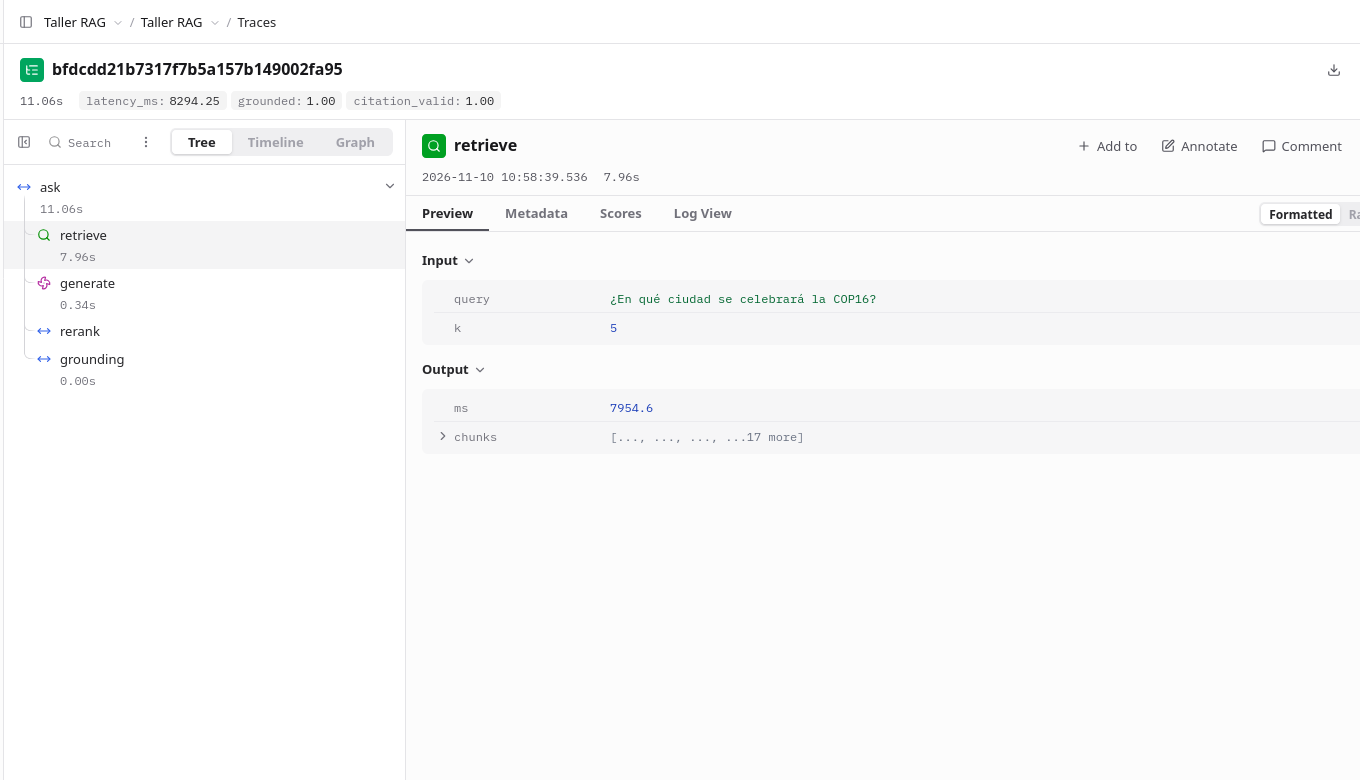
\includegraphics[width=\textwidth]{langfuse_trace_crop.png}
\caption{Traza de una consulta en Langfuse: spans de recuperaci\'on, reordenamiento, generaci\'on y anclaje, con los scores de la petici\'on.}
\label{fig:trace}
\end{figure*}

El conjunto dorado vive como Dataset de Langfuse. Cada corrida es un experimento que enfrenta la respuesta esperada con la respuesta del modelo y calcula cuatro scores por \'item: \texttt{correct}, \texttt{token\_recall}, \texttt{citation\_valid} y \texttt{grounded}. La Figura~\ref{fig:langfuse} muestra la vista de evaluaci\'on con la pregunta, el gold, los scores y la respuesta. La Tabla~\ref{tab:observabilidad} resume las tres corridas sobre las 43 preguntas del silver.

\begin{figure*}[t]
\centering
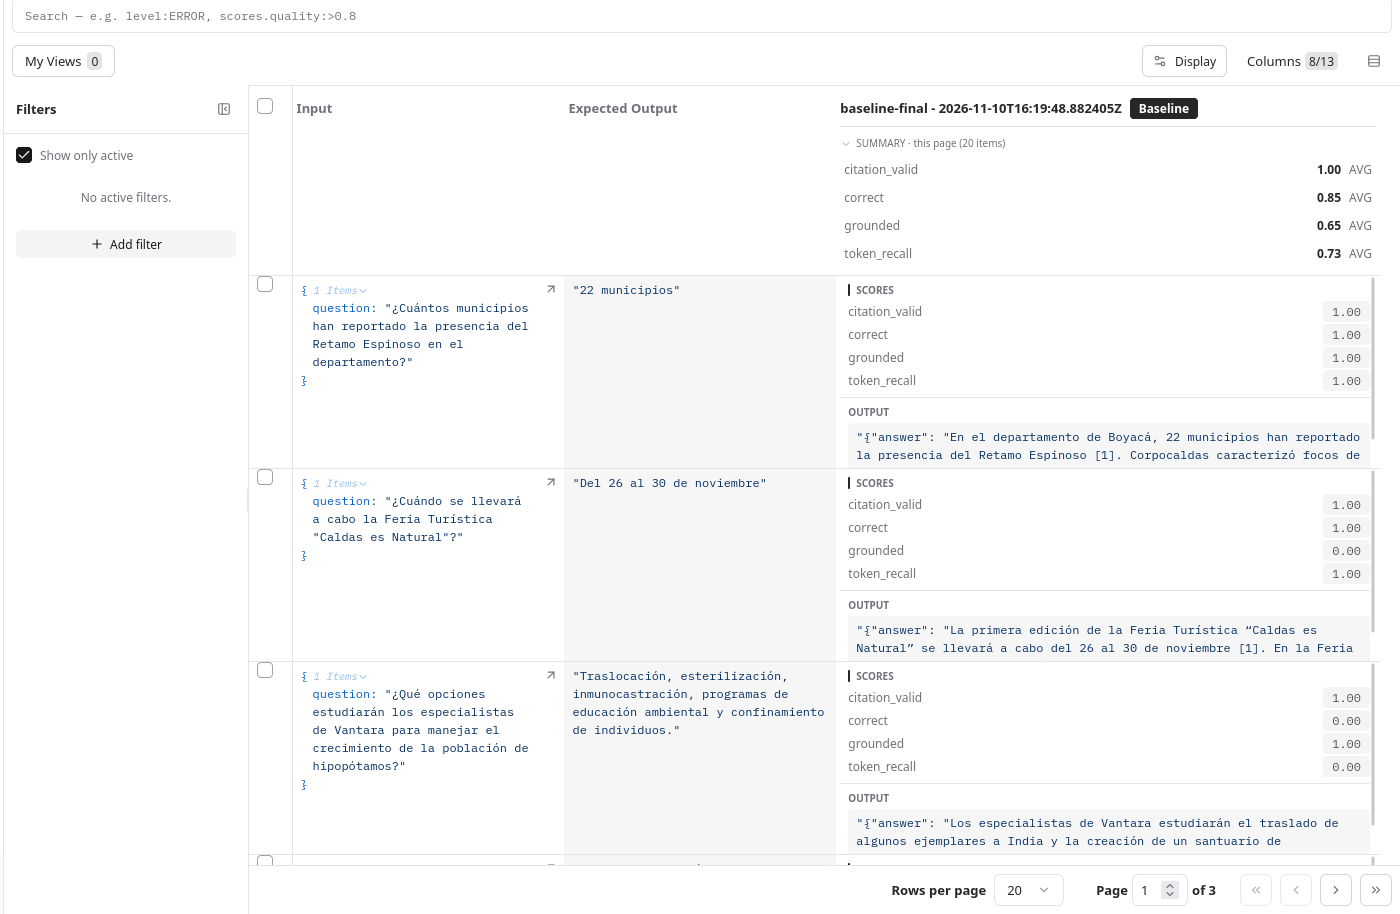
\includegraphics[width=\textwidth]{langfuse_experiment_crop.png}
\caption{Experimento en Langfuse: pregunta, respuesta esperada, scores y respuesta del modelo, con la comparaci\'on por \'item.}
\label{fig:langfuse}
\end{figure*}

\begin{table}[t]
\centering
\footnotesize
\caption{Corridas registradas en Langfuse sobre las 43 preguntas del silver. La exactitud incluye las 5 preguntas sin respuesta.}
\label{tab:observabilidad}
\begin{tabular}{lrrrr}
\toprule
Corrida & Exactitud & Cobertura & Anclaje & p50 \\
\midrule
Uni\'on h\'ibrida & 0,837 & 0,626 & 0,744 & 0,42 s \\
Grafo h\'ibrido & \textbf{0,861} & 0,635 & 0,767 & 1,44 s \\
H\'ibrido + boost & \textbf{0,861} & \textbf{0,655} & \textbf{0,791} & 1,30 s \\
\bottomrule
\end{tabular}
\end{table}

La tabla muestra el efecto de la observabilidad: las tres corridas usan el mismo conjunto, el mismo modelo y la misma temperatura, as\'i que la diferencia es del recuperador. El registro no cambia la respuesta; cambia la capacidad de atribuirla. Sin \'el, una mejora de dos puntos en exactitud no se puede separar de la variaci\'on del muestreo ni del orden de las preguntas.

\subsection{GraphRAG ligero}
\label{sec:graphrag}

Se construy\'o un grafo de documentos y entidades en Neo4j 5.26. Cada documento se conecta con las entidades nombradas que menciona; la extracci\'on corre con spaCy en espa\~nol e ingl\'es sobre el t\'itulo y los primeros 1.500 caracteres. El grafo tiene 169.248 documentos, 248.869 entidades y 926.923 menciones, y se construye en 2.000 s en un solo proceso. La Figura~\ref{fig:neo4j} muestra un documento y sus entidades.

\begin{figure}[t]
\centering
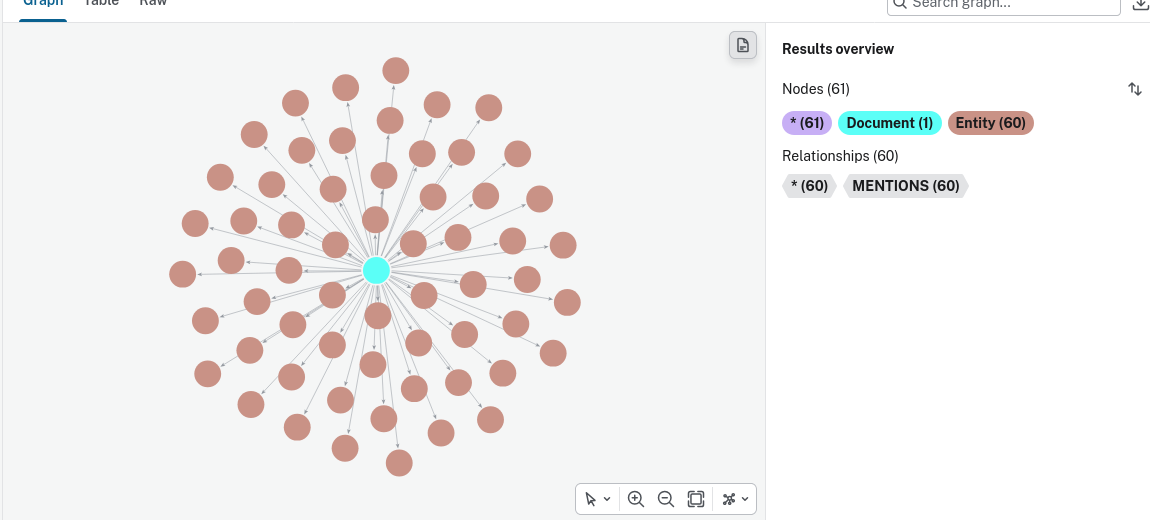
\includegraphics[width=\columnwidth]{neo4j_graph_crop.png}
\caption{Grafo en Neo4j: un documento y las entidades que menciona.}
\label{fig:neo4j}
\end{figure}

Se probaron dos formas de usar el grafo. \texttt{graph\_hybrid} fusiona los candidatos del grafo con la uni\'on densa y BM25 antes del reordenamiento. \texttt{hybrid\_boost} deja intacta la recuperaci\'on y suma al \texttt{rerank\_score} un bono por cada entidad de la consulta presente en el fragmento. La Tabla~\ref{tab:graphrag} compara ambos modos con el baseline en las 43 preguntas y en un conjunto nuevo de 10 preguntas multi-documento.

\begin{table*}[t]
\centering
\footnotesize
\caption{GraphRAG contra la uni\'on h\'ibrida. Exactitud y cobertura de tokens sobre las 43 preguntas del silver y sobre 10 preguntas multi-documento.}
\label{tab:graphrag}
\begin{tabular}{lrrrr}
\toprule
Modo & Exactitud (43) & Cobertura (43) & Exactitud (10) & Cobertura (10) \\
\midrule
Uni\'on h\'ibrida & 0,837 & 0,626 & \textbf{0,900} & 0,878 \\
Grafo h\'ibrido & \textbf{0,861} & 0,635 & 0,700 & 0,694 \\
H\'ibrido + boost & \textbf{0,861} & \textbf{0,655} & \textbf{0,900} & \textbf{0,889} \\
\bottomrule
\end{tabular}
\end{table*}

El resultado separa dos usos que suelen confundirse. El grafo como fuente de candidatos mejora una pregunta en el silver, pero pierde 20 puntos en el conjunto multi-documento: el reordenador prefiere documentos que el grafo trae por entidades ruidosas y desplaza fragmentos que la recuperaci\'on densa ya ten\'ia. El grafo como reordenador, en cambio, sube la cobertura de tokens y el anclaje en ambos conjuntos sin degradar la exactitud. La diferencia es consistente con la calidad de la extracci\'on: las claves no pasan por un enlace de entidades y muchas son frases largas, as\'i que el grafo sirve para desempatar, no para sustituir al \'indice. GraphRAG no es una mejora gratuita; con este corpus y este extractor, el uso defendible es el boost. Se reconstruy\'o el grafo con un filtro de entidades (m\'aximo 4 tokens, sin d\'igitos iniciales, MISC de m\'aximo 3): qued\'o en 206.614 entidades y 852.751 menciones. Con ese grafo y el prompt v3, \texttt{graph\_hybrid} obtiene 0,875 en test y 0,880 en el reservado, mientras el boost obtiene 0,917 y 0,840; en las 10 preguntas multi-documento el grafo sigue en 0,700. La limpieza mejora la precisi\'on del grafo en el reservado, pero no revierte la p\'erdida multi-documento.

\subsection{Mejora de la respuesta y evaluaci\'on sem\'antica}
\label{sec:prompt-v3}

El an\'alisis de errores mostr\'o que la recuperaci\'on no era el \'unico cuello de botella: RAGAS daba 0,947 de cobertura de contexto y 0,607 de correcci\'on. El contexto tra\'ia la evidencia, pero el modelo omit\'ia datos en las preguntas de lista o de dos partes. Se prob\'o un prompt v3 que pide la respuesta directa, todos los datos pedidos y la lista completa, con dos ejemplos y un l\'imite de tres frases. La Tabla~\ref{tab:prompt} compara el prompt v2 y el v3 con el mismo recuperador (uni\'on h\'ibrida m\'as el boost del grafo) en test (24 preguntas) y en el reservado (25).

\begin{table*}[t]
\centering
\footnotesize
\caption{Prompt v2 contra prompt v3 con el mismo recuperador. Exactitud y cobertura de tokens sobre test (24) y el reservado (25).}
\label{tab:prompt}
\begin{tabular}{lrrrr}
\toprule
Configuraci\'on & Exactitud test & Cobertura test & Exactitud reservado & Cobertura reservado \\
\midrule
v2 + boost & \textbf{0,917} & \textbf{0,541} & \textbf{0,840} & \textbf{0,440} \\
v3 + boost & \textbf{0,917} & 0,522 & \textbf{0,840} & \textbf{0,440} \\
v3 sin boost & 0,875 & 0,486 & \textbf{0,840} & \textbf{0,440} \\
\bottomrule
\end{tabular}
\end{table*}

La exactitud es la misma: 0,917 en test y 0,840 en el reservado. La diferencia aparece en la evaluaci\'on sem\'antica. La Tabla~\ref{tab:ragas-v3} repite RAGAS sobre las 19 preguntas respondibles de test y las 20 del reservado. El prompt v3 sube la correcci\'on de 0,590 a 0,652 con el mismo recuperador y la misma exactitud; sin el boost llega a 0,687, a costa de una pregunta exacta. La diferencia pareada es +0,062, IC 95\,\% $[-0{,}019, 0{,}145]$, $p=0{,}14$: con 19 preguntas es una tendencia, no un resultado concluyente. La exactitud no cambia (diferencia 0, IC $[0, 0]$). La fidelidad queda en 1,0 y la cobertura de contexto en 1,0: el generador no inventa y la evidencia alcanza.

\begin{table*}[t]
\centering
\footnotesize
\caption{RAGAS con prompt v2 y v3. Test: 19 preguntas respondibles. Reservado: 20. Juez gemma2:2b y embeddings qwen3-embedding:8b.}
\label{tab:ragas-v3}
\begin{tabular}{lrrrrr}
\toprule
Configuraci\'on & Fidelidad & Relevancia & Precisi\'on & Cobertura & Correcci\'on \\
\midrule
v2 + boost (test) & \textbf{1,000} & \textbf{0,790} & 0,735 & \textbf{1,000} & 0,590 \\
v3 + boost (test) & \textbf{1,000} & 0,772 & 0,728 & \textbf{1,000} & 0,652 \\
v3 + boost (reservado) & 0,938 & 0,798 & 0,808 & \textbf{1,000} & 0,629 \\
v3 sin boost (test) & \textbf{1,000} & 0,799 & \textbf{0,751} & \textbf{1,000} & \textbf{0,687} \\
v3 sin boost (reservado) & 0,975 & \textbf{0,856} & \textbf{0,863} & \textbf{1,000} & 0,655 \\
\bottomrule
\end{tabular}
\end{table*}

La m\'etrica l\'exica subestima las respuestas correctas cuando cambian de idioma. En el reservado, r-012 responde \textit{Foro Econ\'omico Mundial} por \textit{World Economic Forum} y r-019 responde \textit{avispa asi\'atica} por \textit{Asian Hornet}; ambas son correctas y el chequeo de contenci\'on las marca como fallo, mientras RAGAS las punt\'ua por encima de 0,7. Con esa correcci\'on, el reservado pasa de 21 a 23 aciertos sobre 25. La configuraci\'on final es v3 con el boost del grafo: 0,917 de exactitud en test, 0,840 en el reservado, 0,652 de correcci\'on RAGAS en test y 0,629 en el reservado, con 0,938 de fidelidad. El boost no cambia la exactitud del reservado y su efecto en la correcci\'on es +0,030 en test (IC $[-0{,}007, 0{,}074]$, $p=0{,}14$) y +0,010 en el reservado (IC $[-0{,}027, 0{,}065]$, $p=0{,}75$); ninguna de las dos excluye cero. Si se prioriza la correcci\'on sem\'antica sobre una pregunta exacta, v3 sin boost es la mejor opci\'on: 0,687 en test y 0,655 en el reservado, tambi\'en sin diferencia concluyente.

\subsection{Resumen de resultados}

La Figura~\ref{fig:resumen} re\'une los tres resultados principales: RAGAS por configuraci\'on, las pol\'iticas de ambig\"uedad sobre el silver humano y el flujo del conjunto reservado con y sin compuerta.

\begin{figure*}[t]
\centering
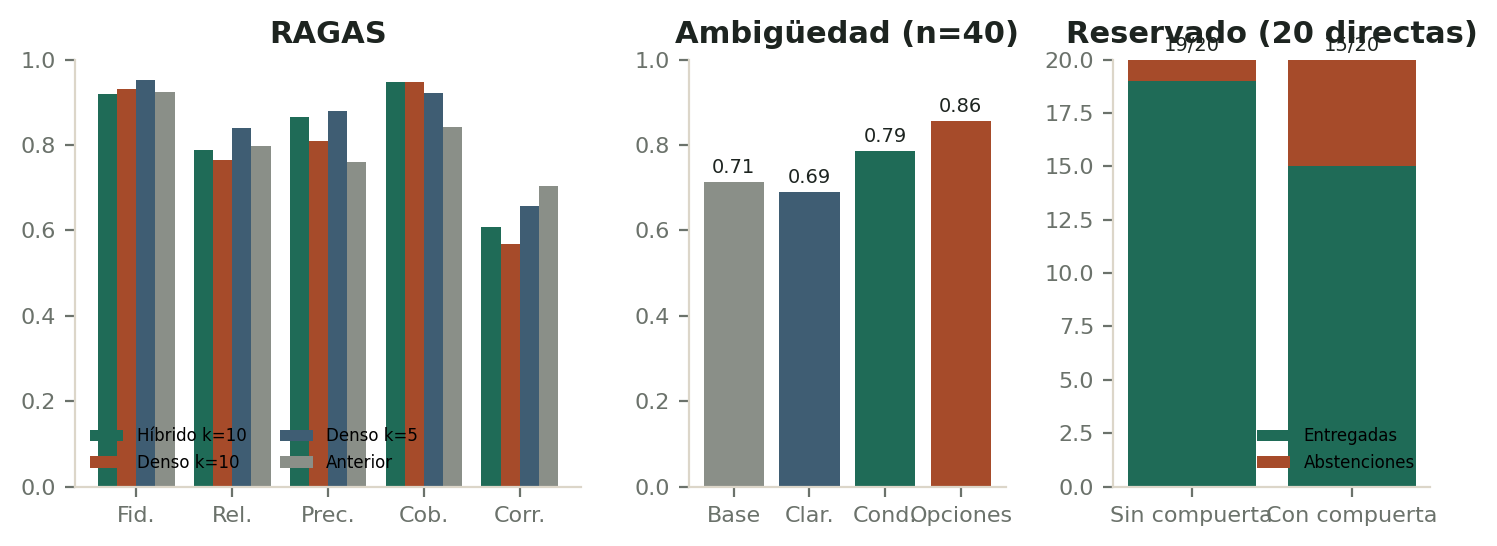
\includegraphics[width=\textwidth]{resumen_final.png}
\caption{Resumen de resultados: RAGAS por configuraci\'on, pol\'iticas de ambig\"uedad y flujo del conjunto reservado con y sin compuerta.}
\label{fig:resumen}
\end{figure*}

\subsection{Conjunto reservado}
\label{sec:reservado}

El silver exploratorio se us\'o para elegir la configuraci\'on densa, as\'i que no mide generalizaci\'on. Se construy\'o un conjunto reservado de 25 preguntas: 20 directas y 5 sin respuesta, 15 en espa\~nol y 10 en ingl\'es, 14 de prensa y 6 de Bluesky. Las preguntas se generaron con Gemma4 y se validaron autom\'aticamente; no son una muestra humana independiente. El conjunto se congel\'o antes de evaluar la compuerta y se us\'o para esa evaluaci\'on. Despu\'es se us\'o tambi\'en para elegir la recuperaci\'on h\'ibrida. Por eso las m\'etricas de recuperaci\'on y respuesta de esta secci\'on son de desarrollo. La compuerta se midi\'o antes de esa elecci\'on, pero el mismo conjunto se us\'o despu\'es para elegir el h\'ibrido: sus cifras tambi\'en son de desarrollo. Una prueba independiente de la recuperaci\'on exige un conjunto nuevo. La Tabla~\ref{tab:reservado} muestra el resultado.

\begin{table}[t]
\centering
\footnotesize
\caption{Conjunto reservado: 20 preguntas directas y 5 sin respuesta, congelado antes de ejecutar; la compuerta se evalu\'o antes de elegir el h\'ibrido.}
\label{tab:reservado}
\begin{tabular}{lrr}
\toprule
M\'etrica & Valor & Denominador \\
\midrule
Recall@10 & 0,700 & 20 \\
nDCG@10 & 0,612 & 20 \\
P@1 & 0,500 & 20 \\
Hit@5 & 0,650 & 20 \\
Cobertura de span & 0,700 & 20 \\
Entregadas & 19 & 20 \\
Abstenciones en directas & 1 & 20 \\
Cobertura de tokens, entregadas & 17 & 19 \\
Cobertura de tokens, todas & 17 & 20 \\
Con cita & 1,000 & 19 \\
Abstenciones en sin respuesta & 5 & 5 \\
Compuerta rechaza & 5 & 5 \\
Latencia media & 6,2 s & 25 \\
Entregadas con compuerta (strict) & 15 & 20 \\
Cobertura de tokens con compuerta & 13 & 15 \\
Rechazos de compuerta & 3 & 20 \\
Rechazos del juez & 2 & 20 \\
\bottomrule
\end{tabular}
\end{table}


Las m\'etricas de respuesta se midieron sin la compuerta estricta; las predicciones de la compuerta se calcularon en una pasada aparte. Con la compuerta activa (\texttt{strict=True}), el flujo conjunto entrega 15 de 20 directas y se abstiene en las 5 negativas: tres directas se rechazan por dominio (r-011, r-012 y r-014) y dos por el juez de evidencia (r-005 y r-006). La cobertura de tokens de las 15 entregadas es 13/15 (0,867). La diferencia con las 19 entregas sin compuerta es el coste del filtro. El recall@10 es 0,700 y el nDCG 0,612, por debajo del 0,912 y 0,818 del silver exploratorio, pero por encima del 0,600 y 0,477 de la recuperaci\'on densa. La uni\'on con BM25 recupera r-012 y r-014, que el denso dejaba fuera, y conserva los aciertos del denso en r-009 y r-013. Seis de las 20 preguntas no recuperan el documento de referencia en el top-10; cuatro se responden correctamente con otro documento que contiene el mismo dato (r-005, r-008, r-017, r-019), una termina en abstenci\'on (r-006) y una es ambigua (r-016). El recall con un solo documento de referencia subestima la recuperaci\'on \'util: la mitad de los fallos de recall no son fallos de respuesta. La profundidad de la uni\'on no es monot\'onica: 20/20 y 30/30 suben el recall@10 a 0,750; 50/50 lo sube a 0,850 y recupera r-006, pero baja las entregas a 18 de 20 y la cobertura de tokens a 16 de 20, porque desplaza evidencia que el modelo usaba bien en r-009 y r-012. La configuraci\'on se queda en 10/20.

La cobertura de tokens entre las entregadas es 17 de 19 (89,5\,\%), y sobre las 20 directas, 17 de 20 (85\,\%). La diferencia con la recuperaci\'on densa est\'a en la uni\'on: recupera las entidades que el denso no trae. En ingl\'es el recall es 0,875 y el nDCG 0,829; en espa\~nol, 0,583 y 0,468. El ingl\'es recupera mejor, al contrario de lo que suger\'ia el silver exploratorio.

Las cinco preguntas sin respuesta se rechazan por la compuerta. En las 20 directas, la compuerta rechaza 3: r-011, r-012 y r-014. r-012 y r-014 son preguntas que la recuperaci\'on h\'ibrida s\'i puede responder, pero la compuerta solo ve el top-5 denso; es una deuda de dise\~no, no un fallo de recuperaci\'on. r-011 s\'i recupera el documento y es un falso rechazo del clasificador. La compuerta nueva baja los falsos rechazos de 6 a 3 y los falsos aceptados de 1 a 0 respecto de la anterior. El 0/9 del conjunto anterior no se confirma como tasa nula, pero el 0/5 tampoco la demuestra.

El fallo m\'as grave es r-006: la pregunta pide los 95 votos en la C\'amara de Representantes y el sistema se abstiene. La evidencia recuperada no contiene la cifra correcta en el top-10, y el modelo prefiere no responder. r-016 es una pregunta ambigua del propio conjunto: no nombra el concierto y el corpus tiene varios; se mantiene en las m\'etricas y se reporta como l\'imite de construcci\'on. r-012 entrega una respuesta evasiva: la evidencia contiene la organizaci\'on, pero el modelo enumera varias iniciativas en lugar de responder World Economic Forum. Es un fallo de generaci\'on, no de recuperaci\'on.

La latencia media del conjunto reservado es 6,2 s (mediana 5,6, p95 9,1), inferior a los 10,8 s de la corrida densa. La uni\'on y el reordenador en GPU compensan el mayor n\'umero de candidatos.

La Tabla~\ref{tab:progresion} resume la progresi\'on de la configuraci\'on. Cada fila es una decisi\'on tomada con una medici\'on, no una preferencia.

\begin{table*}[t]
\centering
\footnotesize
\caption{Progresi\'on de la configuraci\'on y m\'etrica que la justific\'o.}
\label{tab:progresion}
\begin{tabular}{lllll}
\toprule
Etapa & Cambio & Silver & M\'etrica & Decisi\'on \\
\midrule
Piloto & e5-base, 1.932 docs & piloto (38) & Recall@10 0,947 & Punto de partida \\
Escala & corpus completo & 38 & Recall@10 0,684 & El piloto sobreestima \\
Dispersa & BM25 & 38 & Recall@10 0,763 & No alcanza el techo \\
Codificador & bge-m3 & 38 & Recall@10 0,842 & Adoptado \\
\'Indice & \texttt{ef}=800 & 38 & Recall@10 0,895 & Adoptado \\
Fusi\'on & h\'ibrido RRF & 38 & Recall@10 0,895 & Empata, se descarta \\
Fusi\'on & h\'ibrido RRF & ampliado & Recall@10 0,890 & Rechazado \\
Reordenamiento & uni\'on densa+BM25 & reservado (20) & Recall@10 0,700 & Adoptado; recupera parte de la ca\'ida \\
Contexto & $k=10$ & reservado (20) & 19/20 entregadas & Adoptado \\
Prompt & v2 & 38 & 37/38 y cobertura 25/37 & Adoptado \\
Compuerta & 160 preguntas & 20 test & 0 falsos aceptados & Adoptado \\
Fase 6 & cuatro variantes & 38 & sin mejora & Rechazadas \\
Fase 7 & MMR & 38 & recall 0,816 & Rechazado \\
Compuerta & 5 negativas & reservado (5) & 5/5 rechazadas & 3/20 falsos rechazos \\
Prompt & v3 + boost & test (24) & Exactitud 0,917 & Adoptado \\
\bottomrule
\end{tabular}
\end{table*}

